\section{The Definition of a Turing Machine}
\label{sec:def-of-tm}

A \textbf{Turing machine} consists of a \textit{finite control}, a \textit{tape}, and a \textit{head} that can be used for \textit{reading or writing} on that tape.

So the Turing machines seem to form a \textit{stable} and \textit{maximal} class of computational devices, in terms of the computations they can perform. The important points to remember by way of introduction are that Turing machines are designed to satisfy simultaneously these three criteria:
\begin{enumerate}[label=(\alph*)]
  \item They should be automata; that is, their construction and function should be in the same general spirit as the devices previously studied.
  \item They should be as simple as possible to describe, define formally, and reason about.
  \item They should be as general as possible in terms of the computations they can carry out.
\end{enumerate}

In essence, a Turing machine consists of a finite-state control unit and a tape (see Figure 1).
\begin{figure}[H]
  \centering
  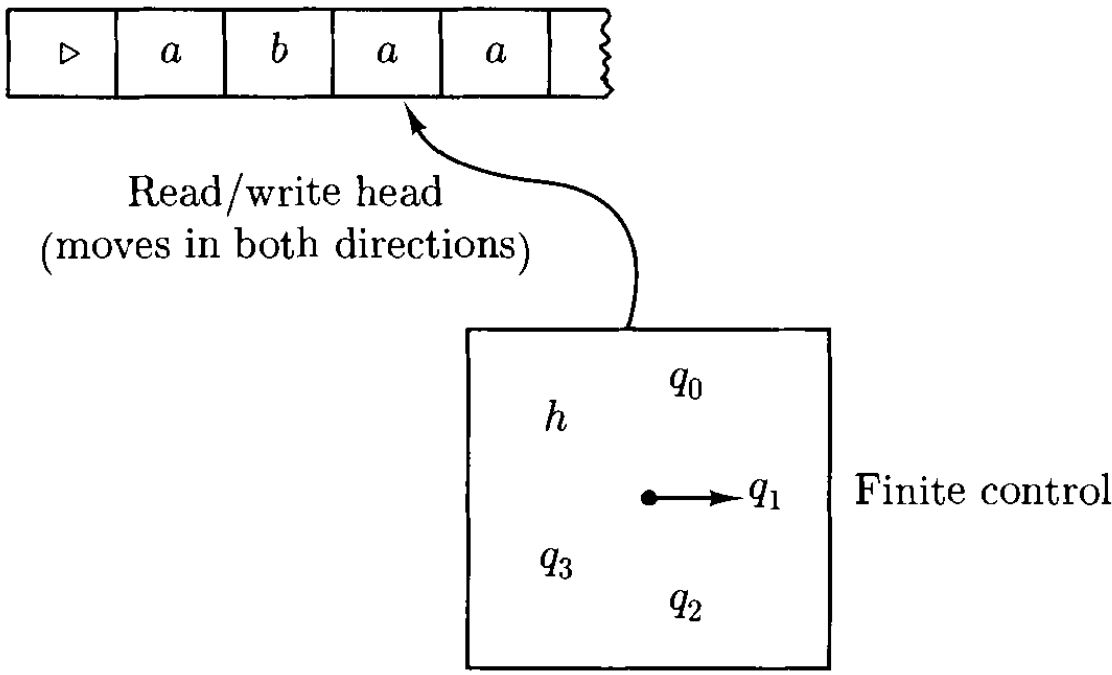
\includegraphics[width=\linewidth]{img/fig-4.1.png}
  \caption{}
  \label{fig:4.1}
\end{figure}
Communication between the two is provided by a single head, which reads symbols from the tape and is also used to change the symbols on the tape. The control unit operates in discrete steps; at each step it performs two functions in a way that depends on its current state and the tape symbol currently scanned by the read/write head:
\begin{enumerate}
  \item Put the control unit in a new state.
  \item Either: 
    \begin{enumerate}
      \item Write a symbol in the tape square currently scanned, replacing the one already there; or
      \item Move the read/write head one tape square to the left or right.
    \end{enumerate}
\end{enumerate}
The tape has a left end, but it extends indefinitely to the right. To prevent the machine from moving its head off the left end of the tape, we assume that the leftmost end of the tape is always marked by a special symbol denoted by $\vartriangleright$; we assume further that all of our Turing machines are so designed that, whenever the head reads a $\vartriangleright$, it immediately moves to the right. Also, we shall use the distinct symbols $\la$ and $\ra$ to denote movement of the head to the left or right; we assume that these two symbols are not members of any alphabet we consider.

A Turing machine is supplied with input by inscribing that input string on tape squares at the left end of the tape, immediately to the right of the $\tar$ symbol. The rest of the tape initially contains \textit{\textbf{blank}} symbols, denoted $\blank$. The machine is free to alter its input in any way it sees fit, as well as to write on the unlimited blank portion of the tape to the right. Since the machine can move its head only one square at a time, after any finite computation only finitely many tape squares will have been visited.

We can now present the formal definition of a Turing machine.
\begin{definition}{}
A Turing machine is a quintuple $(K, \Sigma, \delta, s, H)$, where
\begin{itemize}
  \item $K$ is a \textit{finite set of \textbf{states}};
  \item $\Sigma$ is an \textit{alphabet}, containing the \textit{\textbf{blank symbol}} $\blank$ and the \textit{\textbf{left end symbol}} $\tar$, but not containing the symbols $\la$ and $\ra$;
  \item $s \in K$ is the \textbf{\textit{initial state}};
  \item $H \subseteq K$ is the \textit{set of \textbf{halting states}};
  \item $\delta$, the \textbf{\textit{transition function}}, is a function from $(K - H) \times \Sigma$ to $K \times (\Sigma \cup \{ \la, \ra \})$ such that,
    \begin{enumerate}[label=(\alph*)]
      \item for all $q \in K - H$, if $\delta(q, \tar) = (p, b)$, then $b = \ra$
      \item for all $q \in K - H$ and $a \in \Sigma$, if $\delta(q, a) = (p, b)$ then $b \neq \tar$. 
    \end{enumerate}
\end{itemize}
\end{definition}

If $q \in K - H$, $a \in \Sigma$, and $\delta(q, a) = (p, b)$, then $M$, when in state $q$ and scanning symbol $a$, will enter state $p$, and
\begin{enumerate}
  \item if $b$ is a symbol in $\Sigma$, $M$ will rewrite the currently scanned symbol $a$ as $b$, or 
  \item if $b$ is $\la$ or $\ra$, $M$ will move its head in direction $b$. Since $\delta$ is a function, the operation of $M$ is deterministic and will stop only when $M$ enters a halting state.
\end{enumerate}
Notice these
\begin{itemize}
  \item the requirement (a) on $\delta$: When it sees the left end of the tape $\tar$, it must move right. This way the leftmost $\tar$ is never erased, and $M$ never falls off the left end of its tape.
  \item By (b), $M$ never writes a $\tar$, and therefore $\tar$ is the unmistakable sign of the left end of the tape.
\end{itemize}
In other words, we can think of $\tar$ simply as a ``\textit{protective barrier}'' that prevents the head of $M$ from inadvertently falling off the left end, which does not interfere with the computation of $M$ in any other way. Also notice that $\delta$ is not defined on states in $H$; when the machine reaches a halting state, then its operation stops.

\vspace*{\fill}
\columnbreak

\begin{example}{}
Consider the Turing machine $M = (K, \Sigma, \delta, s, \{h\})$, where
\begin{itemize}
  \item $K = \{ q_0, q_1, h \}$,
  \item $\Sigma = \{ a, \blank, \tar \}$, 
  \item $s = q_0$,
\end{itemize}
and $\delta$ is given by the following table. 
\begin{table}[H]
  \centering
  \begin{tabular}{|cc|c|} 
  \hline
  $q$ & $\sigma$ & $\delta(q, \sigma)$  \\ 
  \hline
  $q_0$  &  $a$       &  $(q_1, \blank)$ \\
  $q_0$  &  $\blank$  &  $(h, \blank)$   \\
  $q_0$  &  $\tar$    &  $(q_0, \ra)$    \\
  $q_1$  &  $a$       &  $(q_0, a)$      \\
  $q_1$  &  $\blank$  &  $(q_0, \ra)$    \\
  $q_1$  &  $\tar$    &  $(q_1, \ra)$    \\
  \hline
  \end{tabular}
\end{table}
\quad When $M$ is started in its initial state $q_0$, it scans its head to the right, changing all $a$'s to $\blank$'s as it goes, until it finds a tape square already containing $\blank$; then it halts. (Changing a nonblank symbol to the blank symbol will be called \textit{\textbf{erasing}} the nonblank symbol.)

\quad To be specific, suppose that $M$ is started with its head scanning the first of four $a$'s, the last of which is followed by a $\blank$. Then $M$ will go back and forth between states $q_0$ and $q_1$ four times, alternately changing an $a$ to a $\blank$ and moving the head right; the first and fifth lines of the table for $\delta$ are the relevant ones during this sequence of moves. 

\quad At this point, $M$ will find itself in state $q_0$ scanning $\blank$ and, according to the second line of the table, will halt. Note that the fourth line of the table, that is, the value of $\delta(q_1, a)$, is irrelevant, since $M$ can never be in state $q_1$ scanning an $a$ if it is started in state $q_0$. Nevertheless, some value must be associated with $\delta(q_1, a)$ since $\delta$ is required to be a function with domain $(K - H) \times \Sigma$.
\end{example}

\begin{example}{}
Consider the Turing machine $M = (K, \Sigma, \delta, s, \{h\})$, where
\begin{itemize}
  \item $K = \{ q_0, h \}$,
  \item $\Sigma = \{ a, \blank, \tar \}$, 
  \item $s = q_0$,
\end{itemize}
\begin{table}[H]
  \centering
  \begin{tabular}{|cc|c|} 
  \hline
  $q$ & $\sigma$ & $\delta(q, \sigma)$  \\ 
  \hline
  $q_0$  &  $a$       &  $(q_0, \la)$ \\
  $q_0$  &  $\blank$  &  $(h, \blank)$   \\
  $q_0$  &  $\tar$    &  $(q_0, \ra)$    \\
  \hline
  \end{tabular}
\end{table}
This machine scans to the left until it finds a $\blank$ and then halts. If every tape square from the head position back to the left end of the tape contains an $a$, and of course the left end of the tape contains a $\tar$, then $M$ will go to the left end of the tape, and from then on it will indefinitely go back and forth between the left end and the square to its right. Unlike other deterministic devices that we have encountered, \textit{the operation of a Turing machine may never stop}.

\end{example}

We now formalize the operation of a Turing machine. To \textit{specify the status} of a Turing machine computation, we need to \textit{specify the state}, the \textit{contents of the tape}, and \textit{the position of the head}. Since all but a finite initial portion of the tape will be blank, the contents of the tape can be specified by a finite string. We choose to break that string into two pieces: 
\begin{itemize}
  \item the part to the left of the scanned square, including the single symbol in the scanned square; and 
  \item the part, possibly empty, to the right of the scanned square.
\end{itemize}
Moreover, so that no two such pairs of strings will correspond to the 
same combination of head position and tape contents, we insist that the second string not end with a blank (all tape squares to the right of the last one explicitly represented are assumed to contain blanks anyway). These considerations lead us to the following definitions.
\begin{definition}{}
  A \textbf{configuration} of a Turing machine $M = (K, \Sigma, \delta, s, H)$ is a member of 
  \begin{equation*}
    K \times \tar\Sigma^* \times (\Sigma^*(\Sigma - \{ \blank \}) \cup \{e\})
  \end{equation*}
\end{definition}
That is, all configurations are assumed to start with the left end symbol, and never end with a blank -unless the blank is currently scanned. Thus $(q, {\tar}a, aba)$, $(h, {\tar}{\blank}{\blank}{\blank}, {\blank}a)$, and $(q, {\tar}{\blank}a{\blank}{\blank}, e)$ are configurations (see Figure 2), but $(q, {\tar}baa, a, bc{\blank})$ and $(q, {\blank}aa, ba)$ are not. A configuration whose state component is in $H$ will be called a \textit{\textbf{halted configuration}}.
\begin{figure}[H]
  \centering
  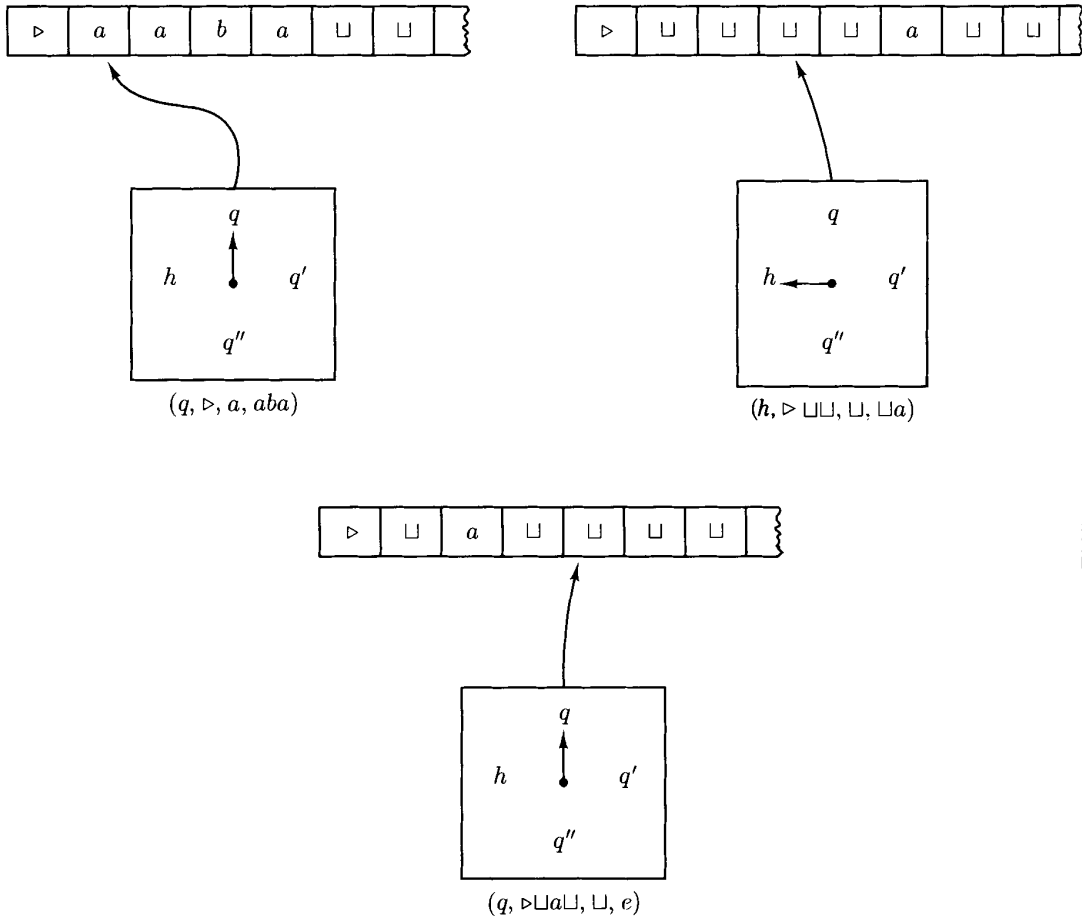
\includegraphics[width=\linewidth]{img/fig-4.2.png}
  \caption{}
  \label{fig:4.2}
\end{figure}
We shall use a simplified notation for depicting the tape contents (including the position of the head): We shall write $w\underline{a}u$ for the tape contents of the configuration $(q, wa, u)$; the underlined symbol indicates the head position. For the three configurations illustrated in Figure 2, the tape contents would be represented as ``${\tar}\underline{a}aba$'', ``${\tar}\blank\blank\underline{\blank}{\blank}a$'', and ``${\tar}{\blank}a{\blank}\underline{\blank}$''.

\vspace*{\fill}
\columnbreak

Also, we can write configurations by including the state together with the notation for the tape and head position. That is, we can write $(q, wa, u)$ as $(q, w\underline{a}u)$. Using this convention, we would write the three configurations shown in Figure 2 as ``$(q, {\tar}\underline{a}aba)$'', ``$(h, {\tar}\blank\blank\underline{\blank}{\blank}a)$'', and ``$(q, {\tar}{\blank}a{\blank}\underline{\blank})$''.
\begin{definition}{}
Let $M = (K, \Sigma, \delta, s, H)$ be a Turing machine and consider two configurations of $M$, $(q_1, w_1\underline{a_1}u_1)$ and $(q_2, w_2\underline{a_2}u_2)$, where $a_1, a_2 \in \Sigma$. Then
\begin{equation*}
  (q_1, w_1\underline{a_1}u_1) \vdash_M (q_2, w_2\underline{a_2}u_2)
\end{equation*}
if and only if, for some $b \in \Sigma \cup \{\la, \ra\}$, $\delta(q_1, a_1) = (q_2, b)$, and either
\begin{enumerate}
  \item $b \in \Sigma$, $w_1 = w_2$, $u_1 = u_2$, and $a_2 = b$, or
  \item $b = \la$, $w_1 = w_2a_2$, and either
    \begin{enumerate}
      \item $u_2 = a_1u_1$, if $a_1 \neq \blank$ or $u_1 \neq e$, or
      \item $u_2 = e$, if $a_1 = \blank$ and $u_1 = e$
    \end{enumerate}
  \item $b = \ra$, $w_2 = w_1a_1$, and either
    \begin{enumerate}
      \item $u_1 = a_2u_2$, or 
      \item $u_1 = u_2 = e$, and $a_2 = \blank$
    \end{enumerate}
\end{enumerate}
\end{definition}
\begin{itemize}
  \item In Case 1, $M$ rewrites a symbol without moving its head.
  \item In Case 2, $M$ moves its head one square to the left; if it is moving to the left off blank tape, the blank symbol on the square just scanned disappears from the configuration.
  \item In Case 3, $M$ moves its head one square to the right; if it is moving onto blank tape, a new blank symbol appears in the configuration as the new scanned symbol.
\end{itemize}
\noindent Notice that all configurations, except for the halted ones, yield exactly one configuration.
\begin{example}{}
To illustrate these cases, let $w, u \in \Sigma^*$, where $u$ does not end 
with a $\blank$, and let $a, b \in \Sigma$.
\begin{itemize}
  \item \textit{Case 1}: $\delta(q_1, a) = (q_2, b)$.
    \begin{itemize}[label={}]
      \item \textit{Example:} $(q_1, w\underline{a}u) \vdash_M (q_2, w\underline{b}u)$.
    \end{itemize}

  \item \textit{Case 2}: $\delta(q_1, a) = (q_2, \la)$.
    \begin{itemize}[label={}]
      \item \textit{Example for (a)}: $(q_1, wb\underline{a}u) \vdash_M (q_2, w\underline{b}au)$.
      \item \textit{Example for (b):} $(q_1, wb\underline{\blank}) \vdash_M (q_2, w\underline{b})$.
    \end{itemize}

  \item \textit{Case 3}: $\delta(q_1, a) = (q_2, \ra)$.
    \begin{itemize}[label={}]
      \item \textit{Example for (a)}: $(q_1, w\underline{a}bu) \vdash_M (q_2, wa\underline{b}u)$.
      \item \textit{Example for (b)}: $(q_1, w\underline{a}) \vdash_M (q_2, wa\underline{\blank})$.
    \end{itemize}
\end{itemize}
\end{example}

\vspace*{\fill}
\columnbreak

\begin{definition}{}
For any Turing machine $M$, let, $\vdash_M^*$ be the reflexive, transitive 
closure of $\vdash_M$; we say that configuration $C_1$ \textbf{yields} configuration $C_2$ if $C_1 \vdash_M^* C_2$. A \textbf{computation} by $M$ is a sequence of configurations $C_0, C_1 , \ldots, C_n$, for some $n \geq 0$ such that
\begin{equation*}
  c_0 \vdash_M C_1 \vdash_M C_2 \vdash_M \cdots \vdash_M C_n
\end{equation*}
\noindent We say that the computation is of length $n$ or that it has $n$ steps, and we write $C_0 \vdash_M^n C_n$.
\end{definition}
Consider the Turing machine $M$ described in Example 1.1. If $M$ is started in configuration $(q_1, {\tar}\underline{\blank}aaaa)$, its computation would be represented formally as follows.
\begin{align*}
  (q_1, {\tar}\underline{\blank}aaaa) 
      &\vdash_M (q_0, {\tar}{\blank}\underline{a}aaa)\\
      &\vdash_M (q_1, {\tar}{\blank}\underline{\blank}aaa)\\
      &\vdash_M (q_0, {\tar}{\blank}\blank\underline{a}aa)\\
      &\vdash_M (q_1, {\tar}{\blank}\blank\underline{\blank}aa)\\
      &\vdash_M (q_0, {\tar}{\blank}\blank\blank\underline{a}a)\\
      &\vdash_M (q_1, {\tar}{\blank}\blank\blank\underline{\blank}a)\\
      &\vdash_M (q_0, {\tar}{\blank}\blank\blank\blank\underline{a})\\
      &\vdash_M (q_1, {\tar}{\blank}\blank\blank\blank\underline{\blank})\\
      &\vdash_M (q_0, {\tar}{\blank}\blank\blank\blank\blank\underline{\blank})\\
      &\vdash_M (h, {\tar}{\blank}\blank\blank\blank\blank\underline{\blank})      
\end{align*}
The computation has 10 steps.

\subsection{A Notation for Turing Machines}

We need a notation for Turing machines that is more graphic and transparent. we shall use a \textit{hierarchical} notation, in which more and more complex machines are built from simpler materials. To this end, we shall define a very simple repertoire of \textit{basic machines}, together with \textit{rules for combining machines}.

\paragraph{\textit{The Basic Machines}.} We start from very humble beginnings: The \textit{symbol-writing machines} and the \textit{head-moving machines}. 

Let us fix the alphabet $\Sigma$ of our machines. For each $a \in \Sigma \cup \{ \ra, \la \} - \{ \tar \}$, we define a Turing machine $M_a = (\{s, h\}, \Sigma, \delta, s, \{h\})$, where for each $b \in \Sigma - \{ \tar \}$, $\delta(s, b) = (h, a)$.

Naturally, $\delta(s, \tar)$ is still always $(s, \ra)$. That is, the only thing this machine does is to perform action a (writing symbol $a$ if $a \in \Sigma$, moving in the direction indicated by $a$ if $a \in \{ \la, \ra \}$) and then to immediately halt.

Naturally, there is a unique exception to this behavior: If the scanned symbol is a $\tar$, then the machine will dutifully move to the right.

Because the symbol-writing machines are used so often, we abbreviate their 
names and write simply $a$ instead of $M_a$. That is, if $a \in \Sigma$, then the $a$-writing machine will be denoted simply as $a$. The head-moving machines $M_{\la}$ and $M_{\ra}$ will be abbreviated as $L$ (for ``\textit{left}'') and $R$ (for ``\textit{right}''). 

\paragraph{\textit{The Rules for Combining Machines}.} Turing machines will be combined in a way suggestive of the structure of a finite automaton. Individual machines are like the states of a finite automaton, and the machines may be connected to each other in the way that the states of a finite automaton are connected together. However, the connection from one machine to another is not pursued until the first machine halts; the other machine is then started from its initial state with the tape and head position as they were left by the first machine. 
\begin{figure}[H]
  \centering
  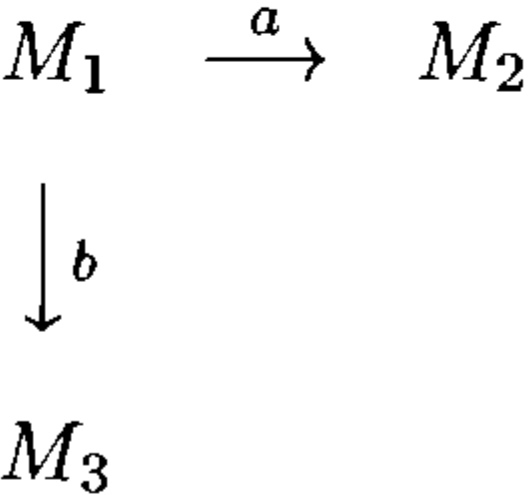
\includegraphics[width=.27\linewidth]{img/fig-4.3.png}
  \caption{}
  \label{fig:4.3}
\end{figure}
So if $M_1$, $M_2$, and $M_3$ are Turing machines, the machine displayed in Figure 3 operates as follows:
\begin{quotation}
  \textit{Start in the initial state of $M_1$; operate as $M_1$ would operate until $M_1$ would halt; then, if the currently scanned symbol is an $a$, initiate $M_2$ and operate as $M_2$ would operate; otherwise, if the currently scanned symbol is a $b$, then initiate $M_3$ and operate as $M_3$ would operate.}
\end{quotation}
Let us take the machine shown in Figure 3 above. Suppose that the three Turing machines $M_1$, $M_2$, and $M_3$ are $M_1 = (K_1, \Sigma, \delta_1, s_1, H_1)$, $M_2 = (K_2, \Sigma, \delta_2, s_2, H_2)$ and $M_3 = (K_3, \Sigma, \delta_3, s_3, H_3)$. We shall assume, as it will be most convenient in the context of combining machines, that the sets of states of all these machines are disjoint. The combined machine shown in Figure 3 above would then be $M = (K, \Sigma, \delta, s, H)$, where
\begin{itemize}[label={}]
  \item $K = K_1 \cup K_2 \cup K_3$,
  \item $s = s_1$,
  \item $H = H_2 \cup H_3$.
  \item For each $\sigma \in \Sigma$ and $q \in K - H$, $\delta(q, \sigma)$ is defined as follows:
    \begin{enumerate}[label=(\alph*)]
      \item If $q \in K_1 - H_1$, then $\delta(q, \sigma) = \delta_1(q, \sigma)$.
      \item If $q \in K_2 - H_2$, then $\delta(q, \sigma) = \delta_2(q, \sigma)$.
      \item If $q \in K_3 - H_3$, then $\delta(q, \sigma) = \delta_3(q, \sigma)$.
      \item Finally, if $q \in H_1$ (the only case remaining) then $\delta(q, \sigma) = s_2$ if $\sigma = a$, $\delta(q, \sigma) = s_3$ if $\sigma = b$, and $\delta(q, \sigma) \in H$ otherwise.
    \end{enumerate}
\end{itemize}

\begin{example}{}
Figure 4(a) illustrates a machine consisting of two copies of $R$. The machine represented by this diagram moves its head right one square; then, if that square contains an $a$, or a $b$, or a $\tar$, or a $\blank$, it moves its head one square further to the right.
\begin{figure}[H]
  \centering
  \begin{minipage}{.40\linewidth}
    \centering
    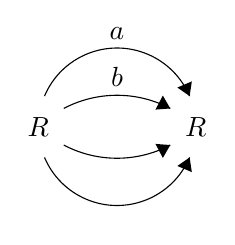
\begin{tikzpicture}[scale=0.2]
      \tikzstyle{every node}+=[inner sep=0pt]
      \draw (0.9,-6.9) node {$R$};
      \draw (10.9,-6.9) node {$R$};
      \draw [black] (1.295,-4.953) arc (-202.91831:-337.08169:5);
      \fill [black] (10.51,-4.95) -- (10.65,-4.02) -- (9.73,-4.41);
      \draw (5.9,-1.4) node [above] {$a$};
      \draw [black] (2.519,-5.737) arc (117.79709:62.20291:7.25);
      \fill [black] (9.28,-5.74) -- (8.81,-4.92) -- (8.34,-5.81);
      \draw (5.9,-4.4) node [above] {$b$};
      \draw [black] (9.281,-8.063) arc (-62.20291:-117.79709:7.25);
      \fill [black] (9.28,-8.06) -- (8.34,-7.99) -- (8.81,-8.88);
      \draw (5.9,-9.4) node [below] {$\tar$};
      \draw [black] (10.505,-8.847) arc (-22.91831:-157.08169:5);
      \fill [black] (10.51,-8.85) -- (9.73,-9.39) -- (10.65,-9.78);
      \draw (5.9,-12.4) node [below] {$\blank$};
    \end{tikzpicture}
    \caption*{(a)}
  \end{minipage}
  \begin{minipage}{.40\linewidth}
    \centering
    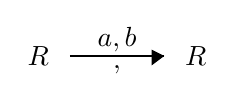
\begin{tikzpicture}[scale=0.2]
      \tikzstyle{every node}+=[inner sep=0pt]
      \draw (0.9,-0.7) node {$R$};
      \draw (10.9,-0.7) node {$R$};
      \draw [black] (2.9,-0.7) -- (8.9,-0.7);
      \fill [black] (8.9,-0.7) -- (8.1,-0.3) -- (8.1,-1.3);
      \draw (5.9,-0.5) node [above] {$a, b$};
      \draw (5.9,-1.3) node [below] {$\tar, \blank$};
    \end{tikzpicture}
    \caption*{(b)}
  \end{minipage}
  \caption{}
  \label{fig:4.4}
\end{figure}
It will be convenient to represent this machine as in Figure 4(b). If an arrow is labeled by \textit{all} symbols in the alphabet $\Sigma$ of the machines, then the labels can be omitted.
\begin{figure}[H]
  \centering
  \begin{minipage}{.3\linewidth}
    \centering
    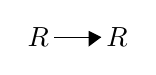
\begin{tikzpicture}[scale=0.2]
      \tikzstyle{every node}+=[inner sep=0pt]
      \draw (0.9,-0.7) node {$R$};
      \draw (5.9,-0.7) node {$R$};
      \draw [black] (1.9,-0.7) -- (4.9,-0.7);
      \fill [black] (4.9,-0.7) -- (4.1,-0.3) -- (4.1,-1.3);
    \end{tikzpicture}
  \end{minipage}
\end{figure}
where, by convention, the leftmost machine is always the initial one. Sometimes an unlabeled arrow connecting two machines can be omitted entirely, by juxtaposing the representations of the two machines. Under this convention, the above machine becomes simply $RR$, or even $R^2$.
\end{example}

\begin{example}{}
If $a \in \Sigma$ is any symbol, we can sometimes eliminate multiple arrows and labels by using $\overline{a}$ to mean ``any symbol except $a$''. Thus, the machine shown in Figure 5(a) scans its tape to the right until it finds a blank. We shall denote this most useful machine by $R_{\blank}$. (The reason why it is named as right scanning is that the label is $R$. If label is $L$, then it is named as scanning to the left.)
\begin{figure}[H]
  \centering
  \begin{minipage}{.49\linewidth}
    \centering
    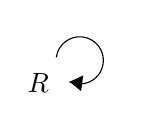
\begin{tikzpicture}[scale=0.2]
      \tikzstyle{every node}+=[inner sep=0pt]
      \draw (0.9,-3.7) node {$R$};
      \draw [black] (2.045,-2.07) arc (172.64789:-115.35211:1.5);
      \draw (5.52,-0.36) node [right] {$\overline{\blank}$};
      \fill [black] (2.89,-3.62) -- (3.62,-4.22) -- (3.75,-3.22);
    \end{tikzpicture}
    \caption*{(a)}
  \end{minipage}
  \begin{minipage}{.49\linewidth}
    \centering
    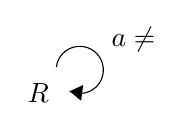
\begin{tikzpicture}[scale=0.2]
      \tikzstyle{every node}+=[inner sep=0pt]
      \draw (0.9,-3.7) node {$R$};
      \draw [black] (2.045,-2.07) arc (172.64789:-115.35211:1.5);
      \draw (5.52,-0.36) node [right] {$a \neq \blank$};
      \fill [black] (2.89,-3.62) -- (3.62,-4.22) -- (3.75,-3.22);
    \end{tikzpicture}
    \caption*{(b)}
  \end{minipage}
  \caption{}
  \label{fig:4.5}
\end{figure}
Another shorthand version of the same machine as in Figure 5(a) is shown 
in Figure 5(b). Here $a \neq \blank$ is read ``any symbol $a$ other than $\blank$''. The advantage of this notation is that a may then be used elsewhere in the diagram as the name of a machine. To illustrate, Figure 6 depicts a machine that scans to the right until it finds a nonblank square, then copies the symbol in that square onto the square immediately to the left of where it was found.
\begin{figure}[H]
  \centering
  \begin{minipage}{.5\linewidth}
    \centering
    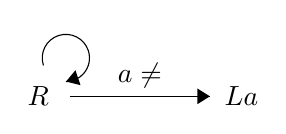
\begin{tikzpicture}[scale=0.2]
      \tikzstyle{every node}+=[inner sep=0pt]
      \draw (0.9,-5.6) node {$R$};
      \draw (13.8,-5.6) node {$La$};
      \draw [black] (1.227,-3.635) arc (198.28227:-89.71773:1.5);
      \draw (4.47,-1.45) node [above] {$\blank$};
      \fill [black] (2.66,-4.66) -- (3.58,-4.89) -- (3.26,-3.94);
      \draw [black] (2.9,-5.6) -- (11.8,-5.6);
      \fill [black] (11.8,-5.6) -- (11,-5.1) -- (11,-6.1);
      \draw (7.35,-5.1) node [above] {$a \neq \blank$};
      \end{tikzpicture}
  \end{minipage}
  \caption{}
\end{figure}
\end{example}

\textit{\textbf{Note:} Check the example 4.1.7 - 4.1.10 from textbook. They are a little basic but important.}
